\section{Project Schedule}
Below is the Gantt chart of our project Schedule. We have planned to perfrom these specific tasks between these time frames.
\begin{figure}[H]
    \centering
        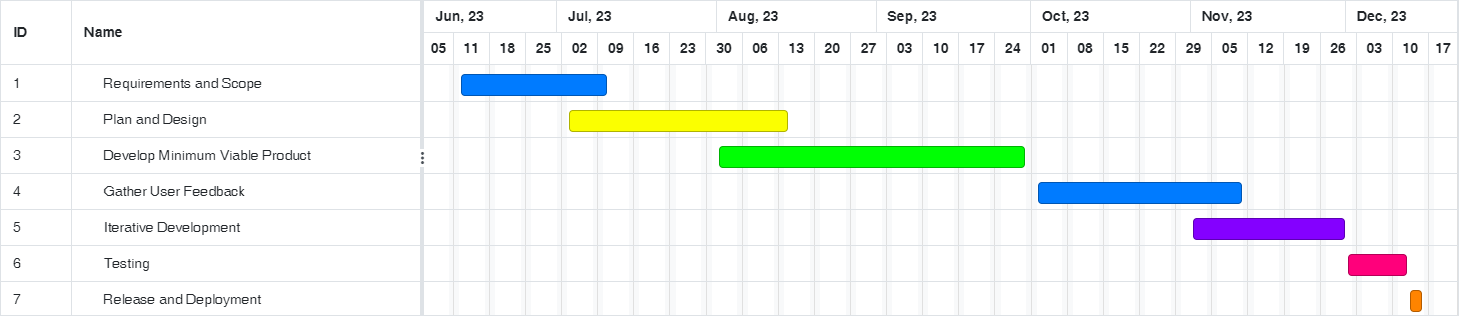
\includegraphics[width=400px]{Diagrams/Gantt_Chart.png}
    \caption{Gantt Chart of Schedule}
\end{figure}

\newpage
\section{Setup Guide to run BuildWizard Locally}
\begin{enumerate}
    \item \textbf{Prerequisite:}
    \begin{enumerate}
        \item XAMPP
        \item Operating System that support XAMPP.
        \item Internet Connection for CDN libraries.
        \item Project Files Cloned from Git Hub.
    \end{enumerate}
    \item Clone Repo in htdocs/\
    \begin{verbatim}
     git clone https://github.com/sujalmhrzn/BuildWizard
    \end{verbatim}
    \item Open PhpMyAdmin by going into \url{http://localhost/phpmyadmin}
    \item Create Database BuildWizard
    \item Import Database sql file from folder cloned using Import button located in navbar.
    \item Open XAMPP Control Panel.
    \item Start Apache and MySQL Servers.
    \item Run it on http://localhost/ Build Wizard directory.
\end{enumerate}
\section{Running Hosted Build Wizard}
\begin{enumerate}
    \item Open Mobile/Desktop Browser .
    \item Go to \url{https://github.com/sujalmhrzn/BuildWizard}
\end{enumerate}
\newpage
\section{MySQL Connection in our Build Wizard PHP}
\vspace{1cm}
\begin{lstlisting}
    <?php
    $servername = "localhost";
    $username = "root";
    $password = "";
    $dbname = "BuildWizard";

    $conn = new mysqli($servername, $username, $password, $dbname);

    if ($conn->connect_error) {
        die("Connection failed: " . $conn->connect_error);
    }
    ?>
    \end{lstlisting}
    \newpage
    \section{Database}
    In the context of the PC part picker project, a database is a structured and organized collection of digital information. It stores essential data such as user profiles and component details.\\
Following figures shows database of users.
\begin{figure}[H]
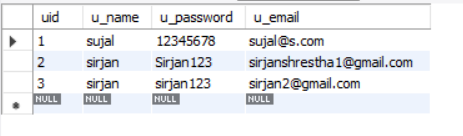
\includegraphics[width=15cm]{Diagrams/Users Database.png}
\caption{User Database}
\end{figure}
Following figures shows components database
\begin{figure}[H]
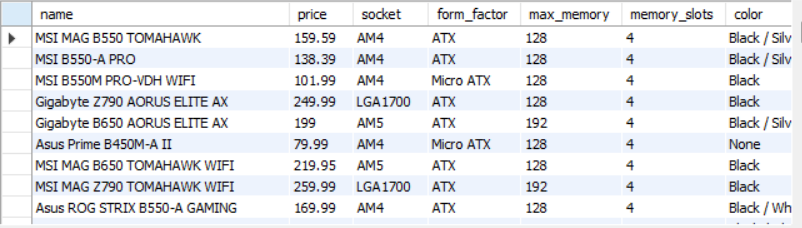
\includegraphics[width=16cm]{Diagrams/motherboard.png}
\caption{Motherboard Database}
\end{figure}
\begin{figure}[H]
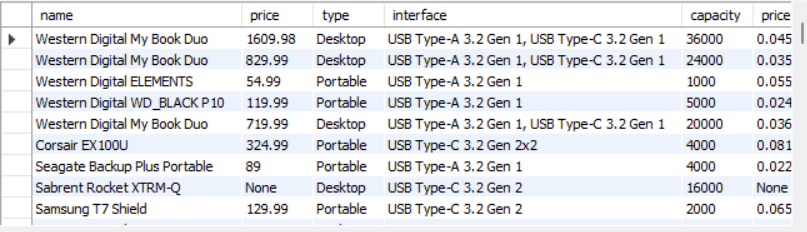
\includegraphics[width=16cm]{Diagrams/External HDD.png}
\caption{External HDD}
\end{figure}

\newpage
\section{Supervisor Consultation Form}
\begin{figure}[H]
    \centering
    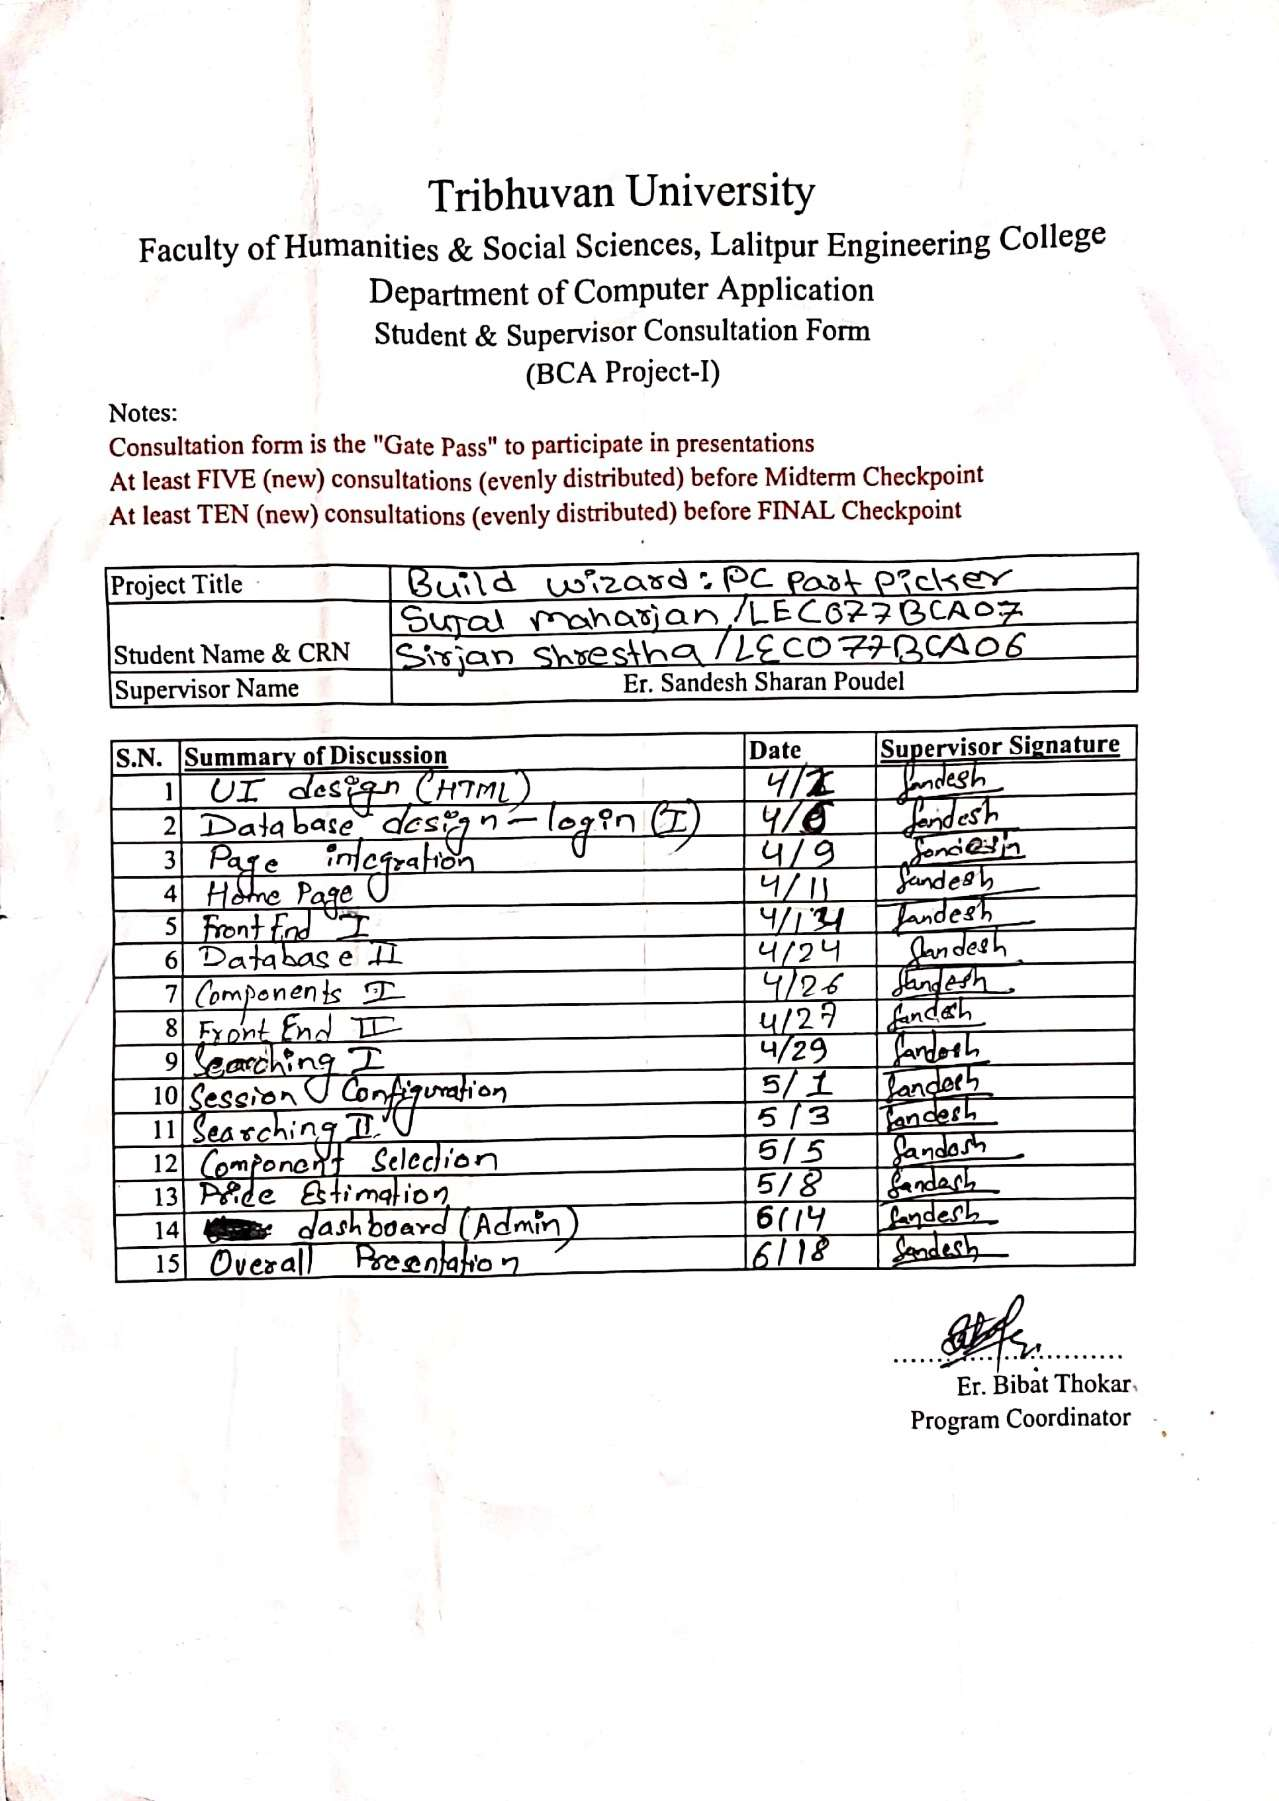
\includegraphics[width=400px]{Diagrams/supervisor.jpg}
\end{figure}


